\subsection{Classification Metrics}

Hypothesis test: Set hypothesis, reject it if $\hat{p}(x) > \tau$ and accept it if $\hat{p}(x) < \tau$

Reject hypothesis $\Rightarrow$ positive | higher $\tau \Rightarrow$ more negatives 



\begin{itemize}
    \item \color{Green}acc.\color{black} = $\frac{TP + TN}{n}$ \hspace{0.1cm} $\bullet$ \color{Green}prec.\color{black}= $ \frac{TP}{TP+FP}$
    \item \color{Red}FPR\color{black} $= \frac{FP}{FP+TN}$ \hspace{0.1cm} $\bullet$ \color{Green}Recall / TPR\color{black}= $\frac{TP}{TP+FN}$
    \item \color{Green}balanced acc.\color{black} $= \frac{1}{n}\sum_iTPR_i$ \hspace{0.1cm} \color{Red}FDR\color{black} = $\frac{FP}{TP + FP}$
    \item \color{Green}F1-score\color{black} = $\underbrace{\frac{2TP}{2TP +FP + FN}}_{\frac{2}{\frac{1}{Recall} + \frac{1}{prec.}}}$ \hspace{0.1cm} \color{Green}ROC\color{black} = $\frac{\text{FPR}}{\text{TPR}}$
\end{itemize}
% ROC curve:
% \begin{multicols*}{2}
%     \begin{center}
%         \resizebox{1\linewidth}{!}{
%         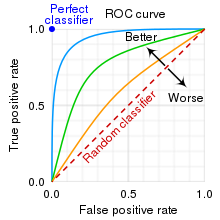
\includegraphics{images/ROC.png}
%         }
%     \end{center}
%     \columnbreak
%     \textbf{ROC} curve is always increasing. Not necessarily convex curve.

%     The higher up the better

%     AUROC = area under ROC

% \end{multicols*}
